\documentclass[10pt,t,xcolor=dvipsnames]{beamer}

\usetheme{Antibes}
\usecolortheme{structure}
%\usepackage[utf8x]{inputenc}
%\usepackage{default}
%\usecolortheme{albatross}
%\usecolortheme{lily}
%\usecolortheme{sidebartab}
%\usecolortheme{crane}
%\usecolortheme{orchid}
%\usecolortheme{albatross}
%\usecolortheme{beetle}
%\usecolortheme{dove}
%\usecolortheme{fly}
%\usecolortheme{seagull}
%\usecolortheme{dolphin}
%\usecolortheme{rose}
\usepackage{graphics}
% \usepackage[pdftex]{graphicx}
\usepackage{graphicx}
\usepackage{xcolor}
\usepackage{color}
%\usepackage{url}
\usepackage{hyperref}
%\usepackage[obeyspaces]{url}
\usepackage{amssymb,amsmath} % for the bold symbol command
\usepackage{booktabs} % toprule etc in tables
\usepackage{mathrsfs}
\usepackage{listings}
\lstset{ %
  backgroundcolor=\color{white},
  basicstyle=\footnotesize,
  breakatwhitespace=false,
  breaklines=true,
  captionpos=b,
  commentstyle=\color{green},
  escapeinside={\%*}{*)},
  extendedchars=true,
  frame=single,
  keywordstyle=\color{blue},
  language=bash,
  numbers=left,
  numbersep=5pt,
  numberstyle=\tiny\color{gray},
  rulecolor=\color{black},
  showspaces=false,
  showstringspaces=false,
  showtabs=false,
  stepnumber=2,
  stringstyle=\color{red},
  tabsize=2,
  title=\lstname,
  morekeywords={not,\},\{,preconditions,effects },
  deletekeywords={time}
}
%\usepackage{minted}
%\usepackage{beamerthemebars}
%\usepackage{ragged2e}
%\usepackage{lipsum}

\setbeamercolor{structure}{fg=RawSienna!50!black}
\renewcommand{\raggedright}{\leftskip=0pt \rightskip=0pt plus 0cm}
\logo{
\includegraphics[scale=0.05]{../../../TWAssets/TW_Colour_Logos_trans_green.png}}

\title{ Introduction to Web Application Development }
\titlegraphic{
\includegraphics[scale=0.15]{../../../TWAssets/TW_Colour_Logos_trans_green.png}}

\author{ Patrick Turley \& 'Wole Solana }
\begin{document}
\nocite*{}
\frame [c, plain]{\titlepage}
%-------------------------------Slide1-------------------------------
\section{Introduction}
\begin{frame}
\frametitle{What is a Web Application?}
\pause
\begin{itemize}[<+->]
\item 1
\item 2
\end{itemize}
\end{frame}
%------------------------------Slide2---------------------------------
\section{Types of Web Frameworks}
\begin{frame}[fragile]
\frametitle{Web Frameworks}
\pause
\begin{itemize}[<+->]
\item 1
\item 2
\item 3
\end{itemize}
\end{frame}
%------------------------------Slide3----------------------------------
\section{The MVC design paradigm}
\begin{frame}[fragile]
\frametitle{Model-View-Controller}
\pause
\begin{itemize}[<+->]
\item 1
% \begin{figure}
% \centering
% 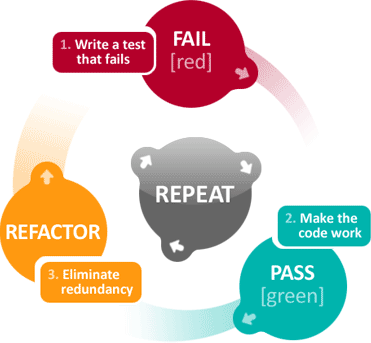
\includegraphics[scale=0.4]{../images/tdd-red-green-refactor-diagram.png}
% \end{figure}
\end{itemize}
\end{frame}
%---------------------------------------------Slide7------------------------------------------------------------------
\section{Further Reading}
\begin{frame}
\frametitle{Further Reading}
% \bibliographystyle{plain}
% \bibliography{DevelopmentPractices.bib}
\end{frame}
\end{document}
